\documentclass[11pt]{article}
\usepackage[utf8]{inputenc}

%%% PAGE DIMENSIONS
\usepackage{geometry}
\geometry{a4paper}

\usepackage{graphicx}

%%% PACKAGES
\usepackage{booktabs}
\usepackage{paralist}
\usepackage{verbatim}
\usepackage{subfig}
\usepackage{chngcntr}
\usepackage{tikz}
\usepackage[colorlinks = true,
            linkcolor = black,
            urlcolor  = blue,
            citecolor = blue,
            anchorcolor = blue]{hyperref}
\usepackage[spanish]{cleveref}
\usepackage{placeins}
\usepackage{float}

%%% HEADERS & FOOTERS
\usepackage{fancyhdr}
\pagestyle{fancy}
\renewcommand{\headrulewidth}{0pt}
\lhead{}\chead{}\rhead{}
\lfoot{}\cfoot{\thepage}\rfoot{}

%%% SECTION TITLE APPEARANCE
\usepackage{sectsty}
\allsectionsfont{\sffamily\mdseries\upshape}

%%% ToC (table of contents) APPEARANCE
\usepackage[nottoc,notlof,notlot]{tocbibind} % Put the bibliography in the ToC
\usepackage[titles,subfigure]{tocloft} % Alter the style of the Table of Contents
\renewcommand{\cftsecfont}{\rmfamily\mdseries\upshape}
\renewcommand{\cftsecpagefont}{\rmfamily\mdseries\upshape} % No bold!


\graphicspath{ {images/} }

\counterwithin*{figure}{section}
\counterwithin*{figure}{subsection}
\counterwithin*{figure}{subsubsection}

\counterwithin*{table}{section}
\counterwithin*{table}{subsection}
\counterwithin*{table}{subsubsection}

\addtolength{\cftfignumwidth}{2em}

\renewcommand{\thefigure}{
  \ifnum\value{subsection}=0
    \thesection.\arabic{figure}
  \else
    \ifnum\value{subsubsection}=0
      \thesubsection.\arabic{figure}
    \else
      \thesubsubsection.\arabic{figure}
    \fi
  \fi
}

\renewcommand{\thetable}{
  \ifnum\value{subsection}=0
    \thesection.\arabic{table}
  \else
    \ifnum\value{subsubsection}=0
      \thesubsection.\arabic{table}
    \else
      \thesubsubsection.\arabic{table}
    \fi
  \fi
}

%%% END Article customizations

%%% The "real" document content comes below...

\title{\Large Seguridad en Redes\\Practica 2.2}
\author{David Antuña Rodríguez\\Javier Carrión García}
\date{}

\begin{document}
  \raggedright

  \maketitle
  \newpage

  \section{OpenSSL}
    \subsection{Creacion de claves RSA, DSA, DH y EC}
      \par
      Hemos adjuntado una carpeta llamada keys que contiene las claves tanto públicas,
      xxpubkey.txt, como privadas, xxkey.txt.

      \bigskip
      \par
      RSA utiliza el teorema chino del resto para precomputar tres valores que aceleran el
      desencriptado del mensaje. Primero veamos cómo desencripta RSA.
      \begin{itemize}
        \item Sean \textbf{p} y \textbf{q} dos numeros primos diferentes escogidos aleatoriamente.
        \item Sea \textbf{n} la longitud de las claves rsa, privada y pública, \textit{n = pq}.
        \item Sea \textbf{d} $\equiv e^{-1}$ mod $\lambda$(n), donde e es un entero tal que 1 $<$
          e $<$ $\lambda$(n).
      \end{itemize}
      Sean m y c el mensaje desencriptado y encriptado, respectivamente.
      \begin{center}
        \Large
        \textit{m = $c^d$ mod n}
      \end{center}

      \par
      Dicho calculo puede resultar muy costoso debido al exponente, d, por lo que se aplica el
      teorema chino del resto para agilizarlo.

      \bigskip
      \par
      En primer lugar se precomputan $d_p$, $d_q$ y $q_{inv}$, con la precondición de que p $>$ q.
      \begin{itemize}
        \item $d_p$ = $e^{-1}$ mod (p-1)
        \item $d_q$ = $e^{-1}$ mod (q-1)
        \item $q_{inv}$ = $q^{-1}$ mod p
      \end{itemize}

      \par
      Una vez se poseen esos valores se pueden realizar los siguientes computos para desencriptar.
      \begin{itemize}
        \item $m_1$ = $c^{d_p}$ mod p
        \item $m_2$ = $c^{d_q}$ mod q
        \item $h$ = $q_{inv}$($m_1$ - $m_2$) mod p
      \end{itemize}

      \par
      Ahora el desencriptado no necesita resolver el exponente que incrementaba su coste.
      \begin{center}
        \Large
        \textit{m = $m_2$ + hq}
      \end{center}

    \subsection{Cifrado y descrifrado con RSA}
      \par
      En la carpeta rsa se encuentra el keyfile cifrado con la clave pública de rsa, keyfile.bin,
      y el resultado de cifrar /etc/services utilizando des3 y el keyfile, cipher.bin.

    \subsection{Firma y verificación con RSA, DSA y EC (ECDSA)}
      \par
      Para todas las firmas se ha empleado el algoritmo de hash sha256.

      \FloatBarrier
      \begin{figure}[H]
        \centering
        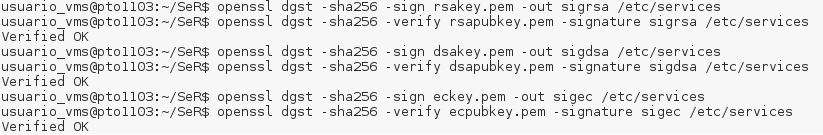
\includegraphics[width = \textwidth]{signs}
        \caption{Firmado y verificado con rsa, dsa y ec.}
      \end{figure}

    \subsection{Acuerdo de claves con DH y EC (ECDH)} \label{ecdh}
      \par
      En la carpeta acuerdos estan los ficheros correspondientes a las nuevas keys y los secretos
      generados.

      \begin{figure}[H]
        \centering
        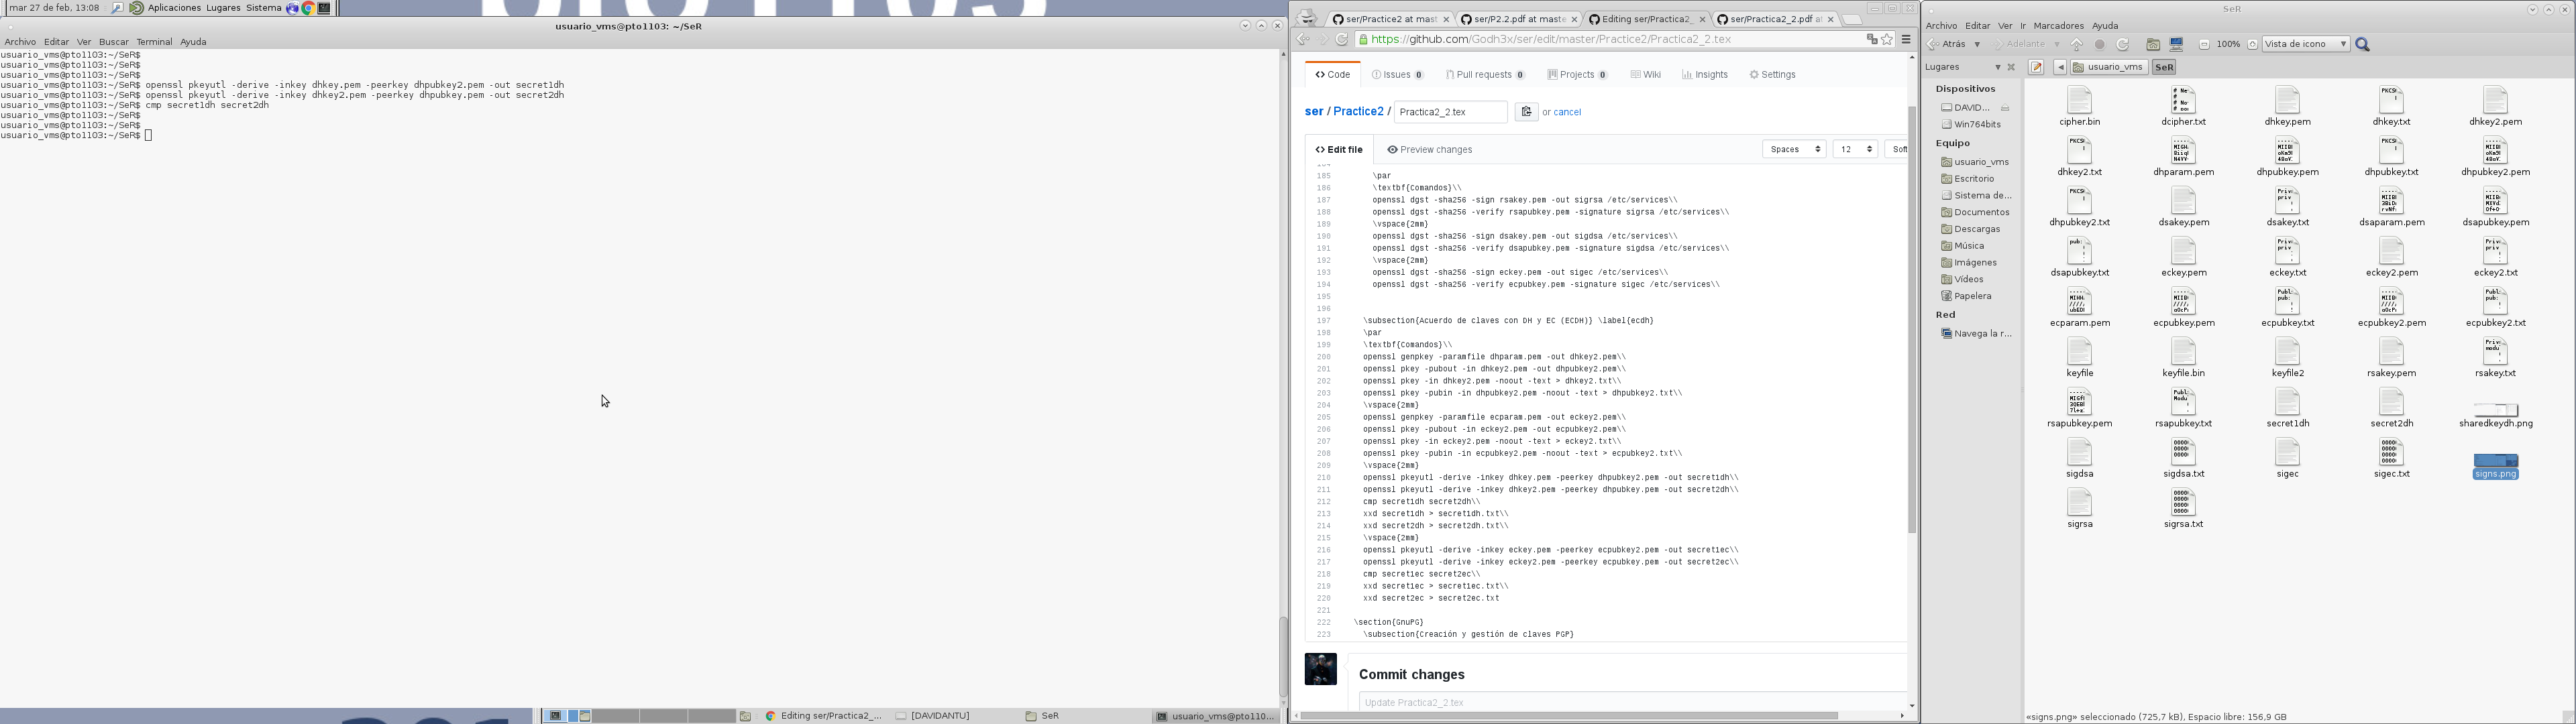
\includegraphics[width = \textwidth]{AcuerdoDH}
        \caption{Acuerdo de claves con DH.}
      \end{figure}

      \begin{figure}[H]
        \centering
        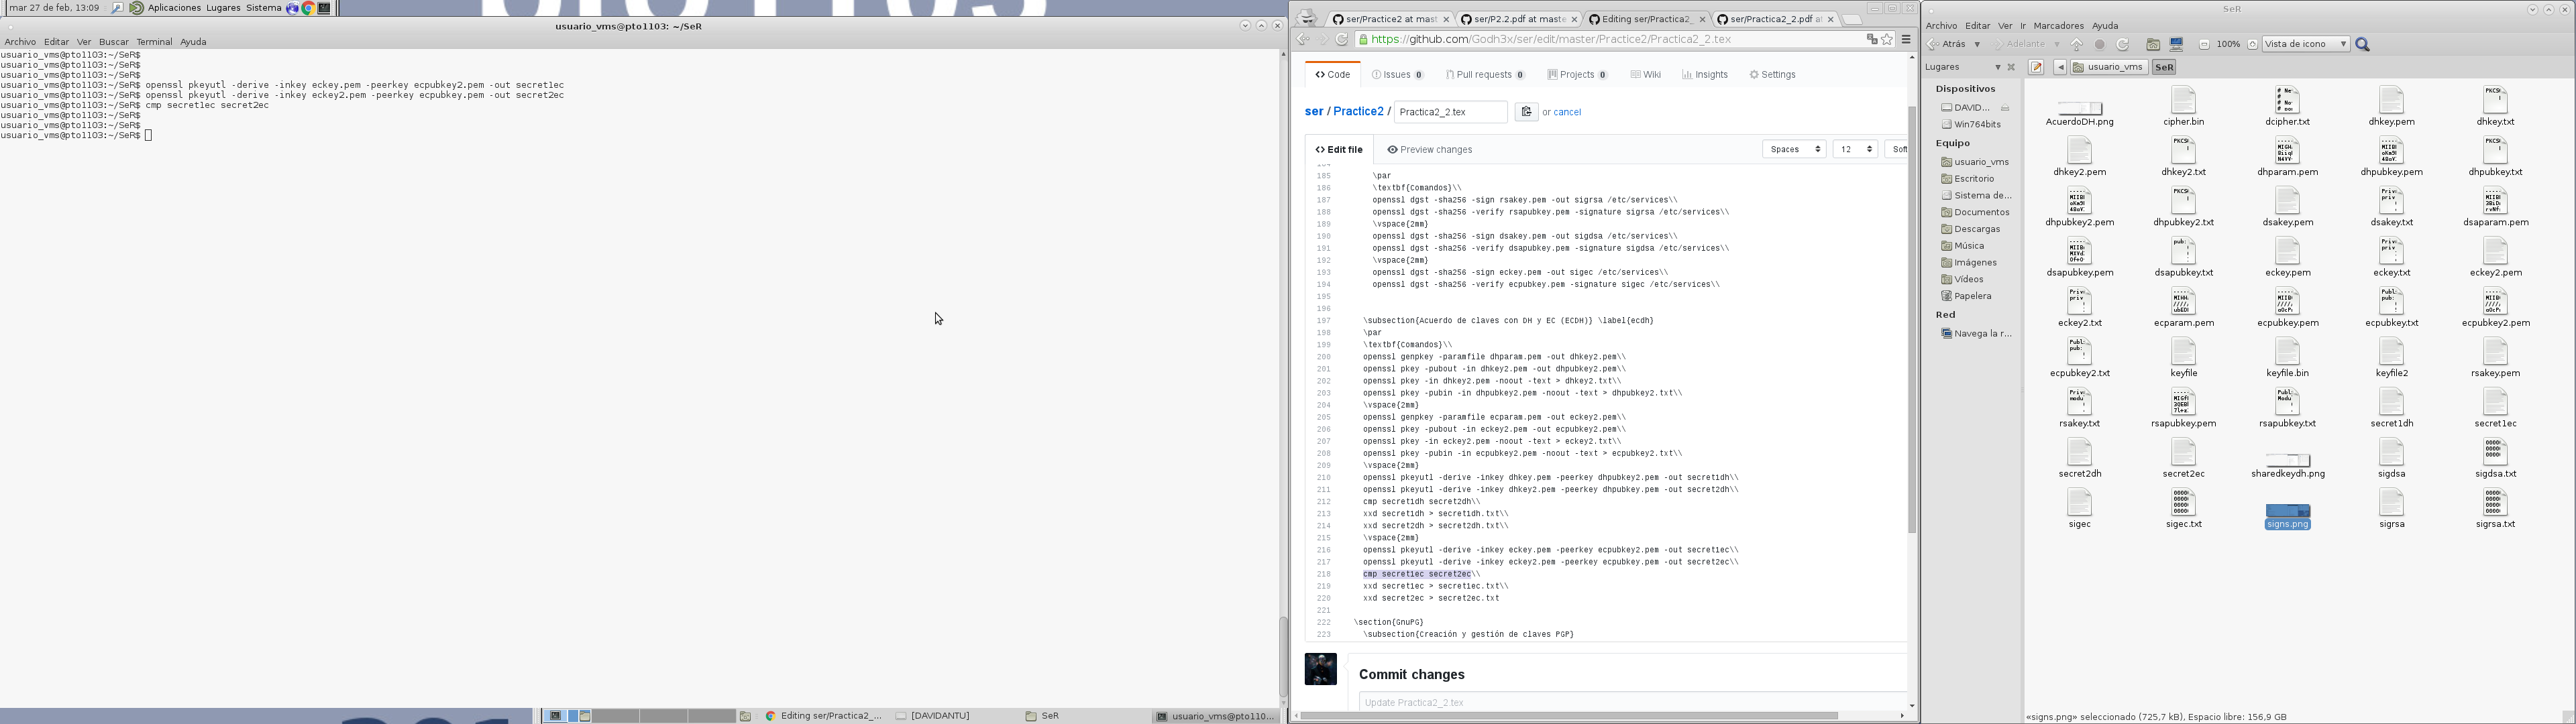
\includegraphics[width = \textwidth]{AcuerdoEC}
        \caption{Acuerdo de claves con EC.}
      \end{figure}

  \section{GnuPG}
    \subsection{Creación y gestión de claves PGP}
      \par
      El id de la clave siempre corresponde al codigo que aparece despues de /, marcado en una de
      las claves de la imagen.

      \begin{figure}[H]
        \centering
        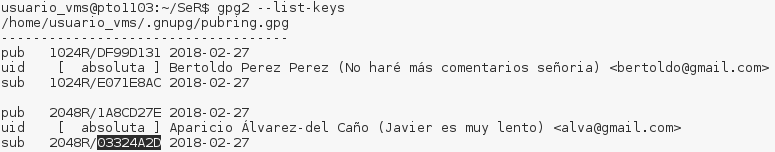
\includegraphics[width = \textwidth]{sring}
        \caption{Claves públicas del anillo.}
      \end{figure}

      \begin{figure}[H]
        \centering
        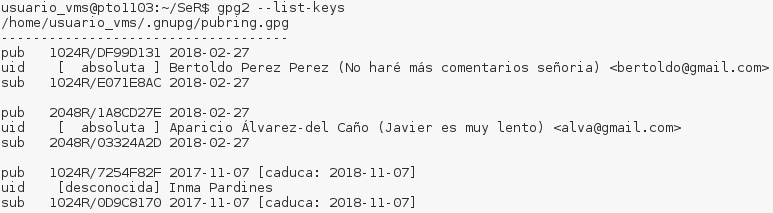
\includegraphics[width = \textwidth]{nring}
        \caption{Claves públicas del anillo tras importar.}
      \end{figure}

    \subsection{Cifrado y descifrado}
      \par
      Hemos cifrado el fichero con la clave pública que has subido al campus.

    \subsection{Firma y verificación}
      \par
      Como se puede ver en la captura hemos probado a cifrar con sha256, esta es la firma que
      hemos entregado, y no hay ningún problema pero si firmamos con md5 no se puede verificar
      porque es un algoritmo no seguro.

      \begin{figure}[H]
        \centering
        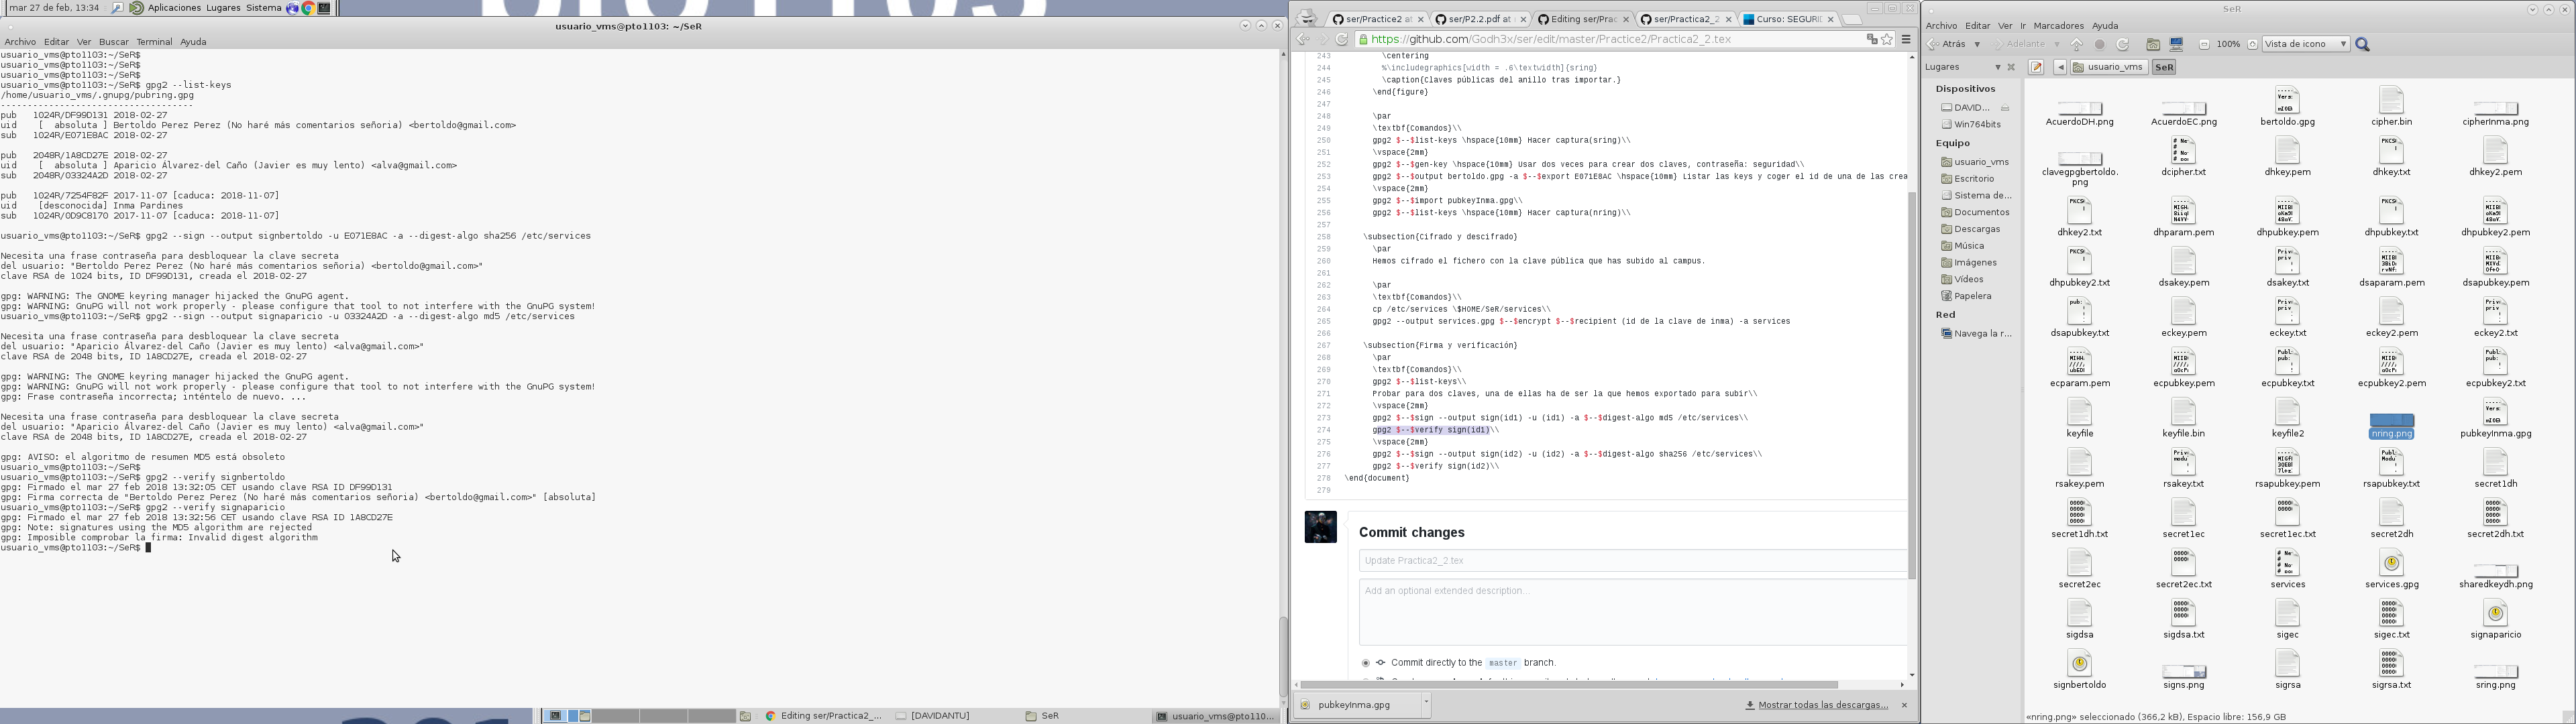
\includegraphics[width = \textwidth]{signverify}
        \caption{Firma y verificacion para Bertoldo y Aparicio.}
      \end{figure}

      \par
      El fichero gpg contiene la clave pública de Bertoldo.
\end{document}
